\chapter{Conclusion and Future Work}
\label{conclusions}
\linenumbers

\paragraph{Discussion}
\label{par:7_discussion}
At this stage, we have completed our (partial) reverse engineering of the iTrust SWaT System, aiming to achieve a sufficient level of the physical process, or \textit{process comprehension}. This \textit{process comprehension} enables us to plan a targeted attack on the system using the information obtained through the dynamic analysis conducted with the framework outlined in Chapter \ref{chap:proposal}, employing a black box approach.

To evaluate the accuracy of the information obtained about the SWaT system, we can refer to Figure \ref{fig:7_swat_schema} \cite{swat_tecnical_pdf}, which provides a schematic representation of the SWaT system. An \texttt{x} indicates placement of sensors. By comparing the information derived from our analysis with the system schematic, we can assess the validity and reliability of our findings.

\begin{figure}[ht]
	\centering
	\includegraphics[scale=0.20]{chap7/swat_schema_1.png}
	\caption{iTrust SWaT schema}
	\label{fig:7_swat_schema}
\end{figure}

\bigskip
This image, while not comprehensive, serves to validate the accuracy of the properties derived from our system analysis of the first four stages of the SWaT system. It demonstrates that we have successfully identified the actuators and sensors within the system, and in some cases, we have even determined their specific roles within the physical process.

\bigskip
Figure \ref{fig:7_swat_hmi} \cite{swat_tecnical_pdf} provides an alternative representation of the SWaT system from the perspective of the Human-Machine Interface (HMI). This depiction complements the previous diagram by adding more contextual information and enhancing overall understanding of the system. It offers a comprehensive view of the system's components and their relationships, thereby improving the clarity and comprehension of the system's structure and functioning.

\begin{figure}[ht]
	\centering
	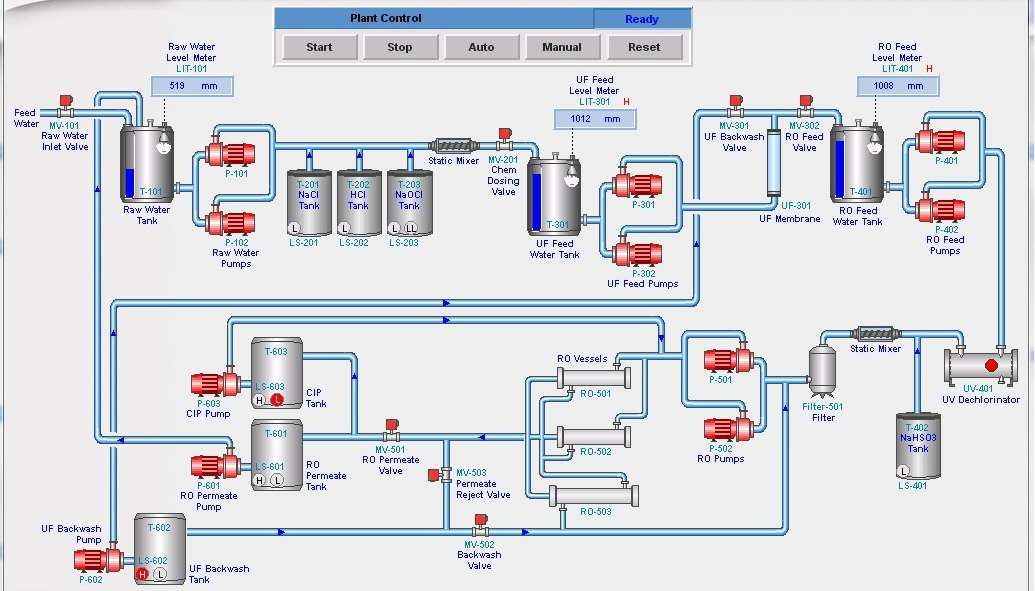
\includegraphics[scale=0.52]{chap7/hmi_swat.jpg}
	\caption{iTrust SWaT schema from HMI point of view.}
	\label{fig:7_swat_hmi}
\end{figure}

\bigskip
This figure introduces additional elements that were not included in the previous schematic shown in Figure \ref{fig:7_swat_schema}. It incorporates spare actuators and other components such as chemical tanks and the ultrafiltration membrane, which were not explicitly represented as registers in the available datasets. A comprehensive list of sensors and actuators, along with their respective functions within the system, can be found in the paper by Adepu et al. \cite{swat_dataset2015}.

However, this figure also serves as further confirmation of the effectiveness of our analysis and the robustness of the framework we employed. Thus, we can confidently assert that \textbf{we have successfully achieved the objectives of this thesis}. We have not only validated the reverse engineering methodology introduced by Ceccato et al., but also improved and enhanced it through its practical application, making it more adaptable and valuable in real-world contexts.

\paragraph{Future work}
\label{par:7_futurework}
The framework, along with the thesis sources and analysis files, is openly accessible on the dedicated GitHub repository. There is potential for further improvement and expansion of the framework. One possibility is integrating the analysis framework with an additional framework that utilizes the gathered data to generate targeted system attacks, building upon the writer's previous work as described in Section \ref{subsec:3_scan_preproc}.

Moreover, the proposed framework can benefit from various improvements and the introduction of specific new features to enhance its capabilities and effectiveness in analyzing industrial control systems. Here are some potential avenues for future work and enhancements to consider:

\begin{itemize}
	\item enhance the scanning and data gathering phase by reimplementing it to include support for multiple industrial protocols, in addition to Modbus. This improvement would enable the framework to detect and communicate with PLCs using various protocols commonly used in ICS environments, expanding its compatibility and usability;
	
	\item enhance the automatic recognition of sensors and actuators by leveraging advanced machine learning and artificial intelligence techniques. This improvement would involve training models to accurately identify and classify different types of sensors and actuators based on their data patterns and characteristics;
	
	\item complete the implementation of network traffic data within the Business Process part of the framework. However, it is crucial to ensure that the network traffic data and physical process data used for analysis are reliable and not compromised by external attackers, as accurate and untampered data is essential for effective analysis;
	
	\item implement an automated system for recognizing real system configurations by excluding actuators that do not significantly contribute to changing the system behavior within the analyzed PLC. This automatic recognition system can save time and effort by eliminating the need to manually filter out non-contributing actuators during the analysis process.
\end{itemize}

\vfill
\nolinenumbers